% Options for packages loaded elsewhere
% Options for packages loaded elsewhere
\PassOptionsToPackage{unicode}{hyperref}
\PassOptionsToPackage{hyphens}{url}
\PassOptionsToPackage{dvipsnames,svgnames,x11names}{xcolor}
%
\documentclass[
  a4paper,
  10pt]{article}
\usepackage{xcolor}
\usepackage{amsmath,amssymb}
\setcounter{secnumdepth}{5}
\usepackage{iftex}
\ifPDFTeX
  \usepackage[T1]{fontenc}
  \usepackage[utf8]{inputenc}
  \usepackage{textcomp} % provide euro and other symbols
\else % if luatex or xetex
  \usepackage{unicode-math} % this also loads fontspec
  \defaultfontfeatures{Scale=MatchLowercase}
  \defaultfontfeatures[\rmfamily]{Ligatures=TeX,Scale=1}
\fi
\usepackage{lmodern}
\ifPDFTeX\else
  % xetex/luatex font selection
\fi
% Use upquote if available, for straight quotes in verbatim environments
\IfFileExists{upquote.sty}{\usepackage{upquote}}{}
\IfFileExists{microtype.sty}{% use microtype if available
  \usepackage[]{microtype}
  \UseMicrotypeSet[protrusion]{basicmath} % disable protrusion for tt fonts
}{}
\makeatletter
\@ifundefined{KOMAClassName}{% if non-KOMA class
  \IfFileExists{parskip.sty}{%
    \usepackage{parskip}
  }{% else
    \setlength{\parindent}{0pt}
    \setlength{\parskip}{6pt plus 2pt minus 1pt}}
}{% if KOMA class
  \KOMAoptions{parskip=half}}
\makeatother
% Make \paragraph and \subparagraph free-standing
\makeatletter
\ifx\paragraph\undefined\else
  \let\oldparagraph\paragraph
  \renewcommand{\paragraph}{
    \@ifstar
      \xxxParagraphStar
      \xxxParagraphNoStar
  }
  \newcommand{\xxxParagraphStar}[1]{\oldparagraph*{#1}\mbox{}}
  \newcommand{\xxxParagraphNoStar}[1]{\oldparagraph{#1}\mbox{}}
\fi
\ifx\subparagraph\undefined\else
  \let\oldsubparagraph\subparagraph
  \renewcommand{\subparagraph}{
    \@ifstar
      \xxxSubParagraphStar
      \xxxSubParagraphNoStar
  }
  \newcommand{\xxxSubParagraphStar}[1]{\oldsubparagraph*{#1}\mbox{}}
  \newcommand{\xxxSubParagraphNoStar}[1]{\oldsubparagraph{#1}\mbox{}}
\fi
\makeatother


\usepackage{longtable,booktabs,array}
\newcounter{none} % for unnumbered tables
\usepackage{calc} % for calculating minipage widths
% Correct order of tables after \paragraph or \subparagraph
\usepackage{etoolbox}
\makeatletter
\patchcmd\longtable{\par}{\if@noskipsec\mbox{}\fi\par}{}{}
\makeatother
% Allow footnotes in longtable head/foot
\IfFileExists{footnotehyper.sty}{\usepackage{footnotehyper}}{\usepackage{footnote}}
\makesavenoteenv{longtable}
\usepackage{graphicx}
\makeatletter
\newsavebox\pandoc@box
\newcommand*\pandocbounded[1]{% scales image to fit in text height/width
  \sbox\pandoc@box{#1}%
  \Gscale@div\@tempa{\textheight}{\dimexpr\ht\pandoc@box+\dp\pandoc@box\relax}%
  \Gscale@div\@tempb{\linewidth}{\wd\pandoc@box}%
  \ifdim\@tempb\p@<\@tempa\p@\let\@tempa\@tempb\fi% select the smaller of both
  \ifdim\@tempa\p@<\p@\scalebox{\@tempa}{\usebox\pandoc@box}%
  \else\usebox{\pandoc@box}%
  \fi%
}
% Set default figure placement to htbp
\def\fps@figure{htbp}
\makeatother





\setlength{\emergencystretch}{3em} % prevent overfull lines

\providecommand{\tightlist}{%
  \setlength{\itemsep}{0pt}\setlength{\parskip}{0pt}}



 
\usepackage[style=apa]{biblatex}
\addbibresource{references.bib}


\usepackage{color}
\usepackage{graphicx}
\usepackage{listings}
\usepackage{lmodern}
\usepackage{mdframed}
\usepackage{url}
\usepackage{needspace}
\linespread{1.25}
\definecolor{blue}{rgb}{0,0,0.8}
\definecolor{dkgreen}{rgb}{0,0.6,0}
\definecolor{mauve}{rgb}{0.58,0,0.82}
\definecolor{gray}{rgb}{0.5,0.5,0.5}
\makeatletter
\@ifpackageloaded{caption}{}{\usepackage{caption}}
\AtBeginDocument{%
\ifdefined\contentsname
  \renewcommand*\contentsname{Table of contents}
\else
  \newcommand\contentsname{Table of contents}
\fi
\ifdefined\listfigurename
  \renewcommand*\listfigurename{List of Figures}
\else
  \newcommand\listfigurename{List of Figures}
\fi
\ifdefined\listtablename
  \renewcommand*\listtablename{List of Tables}
\else
  \newcommand\listtablename{List of Tables}
\fi
\ifdefined\figurename
  \renewcommand*\figurename{Figure}
\else
  \newcommand\figurename{Figure}
\fi
\ifdefined\tablename
  \renewcommand*\tablename{Table}
\else
  \newcommand\tablename{Table}
\fi
}
\@ifpackageloaded{float}{}{\usepackage{float}}
\floatstyle{ruled}
\@ifundefined{c@chapter}{\newfloat{codelisting}{h}{lop}}{\newfloat{codelisting}{h}{lop}[chapter]}
\floatname{codelisting}{Listing}
\newcommand*\listoflistings{\listof{codelisting}{List of Listings}}
\makeatother
\makeatletter
\makeatother
\makeatletter
\@ifpackageloaded{caption}{}{\usepackage{caption}}
\@ifpackageloaded{subcaption}{}{\usepackage{subcaption}}
\makeatother
\usepackage{bookmark}
\IfFileExists{xurl.sty}{\usepackage{xurl}}{} % add URL line breaks if available
\urlstyle{same}
% fallback for those not using the hyperref driver hyperxmp:
\makeatletter
\@ifundefined{xmpquote}{\newcommand{\xmpquote}[1]{#1}}{}
\makeatother
\hypersetup{
  colorlinks=true,
  linkcolor={blue},
  filecolor={Maroon},
  citecolor={Blue},
  urlcolor={Blue},
  pdfcreator={LaTeX via pandoc}}


\author{}
\date{}
\begin{document}

\renewcommand*\contentsname{Table of contents}
{
\setcounter{tocdepth}{3}
\tableofcontents
}

================================================================================

NODE MAP OVERVIEW \& MULTI-MEDIA BLUEPRINT

===========================================================================

\section{Sub-Topic 1: Connecting Metaverse Ethics to Information Ethics
(\textasciitilde300
Words)}\label{sub-topic-1-connecting-metaverse-ethics-to-information-ethics-300-words}

\subsection{Node 1.1: The Metaverse as an embodiment space: Datafication
vs.~Stewardship}\label{node-1.1-the-metaverse-as-an-embodiment-space-datafication-vs.-stewardship}

\begin{itemize}
\item
  \textbf{Provocative Hook}: Is the Metaverse an expansion of human
  freedom, or a raw data prison?
\item
  \textbf{Core IE Motivated Argument}: Information Ethics (IE) views
  virtual reality as an extension of Floridi's \emph{infosphere} where
  informational ``beings'' exist
  \autocite{himmaHandbookInformationComputer2008}. Instead of an amoral
  playground, users enter as \emph{homo poieticus}---creative stewards
  duty-bound to prevent informational \emph{entropy} (the corruption of
  reality and truth) \autocite{himmaHandbookInformationComputer2008}.
  The core ethical dilemma is whether the Metaverse fosters human
  flourishing or commodifies human existence into data streams, a
  tension explored by
  \autocite{capurroOntologicalFoundationInformation2006}.
\item
  \textbf{Multi-Media Cue}: Guided numbered picture scroll of a preamble
  to second life economy, scandal 1, then scandal 2. Captions are placed
  under pictures to explain.

  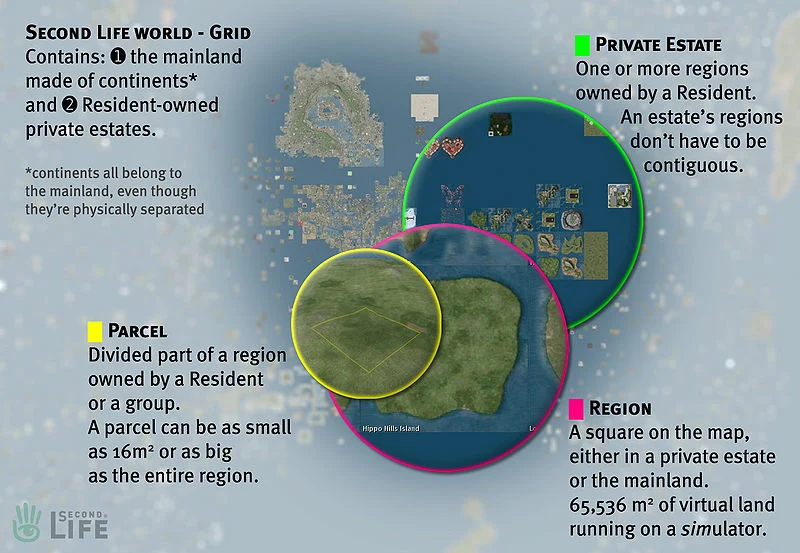
\includegraphics[width=3.125in,height=\textheight,keepaspectratio,alt={As per their website, Second Life features a virtual economy for in game business and real estate management. Currency can be legally converted back into US dollars.}]{images/paste-1.png}\\
  \autocite{lindenBuyingLand2011}\strut \\
  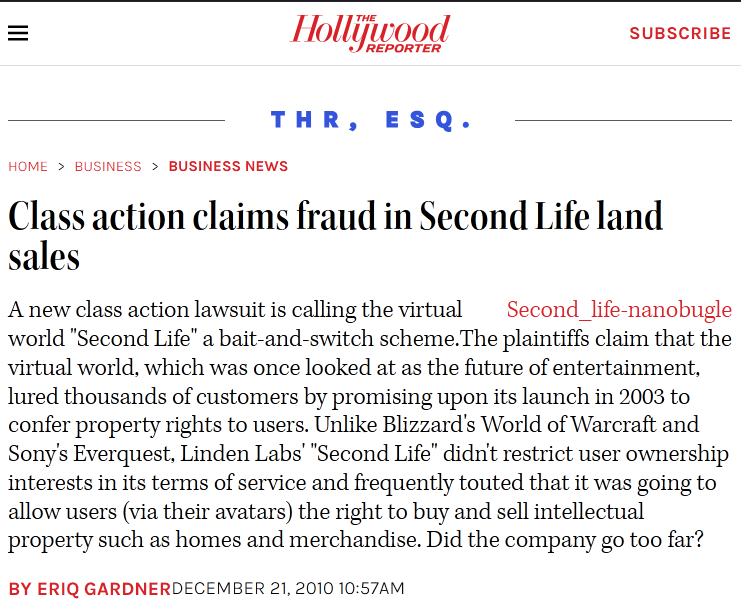
\includegraphics[width=3.125in,height=\textheight,keepaspectratio,alt={The Class Action Property Rights Lawsuit (Amado v. Linden Lab). After allegedly promising true ownership to players, then changing pricing models for land maintenance, players filed a class action Lawsuit. Linden Lab eventually settled, quietly altering their Terms of Service to clarify that players only own a ``limited license'' to access the grid.}]{images/paste-2.png}\\
  \autocite{gardnerClassActionClaims2010}\strut \\
  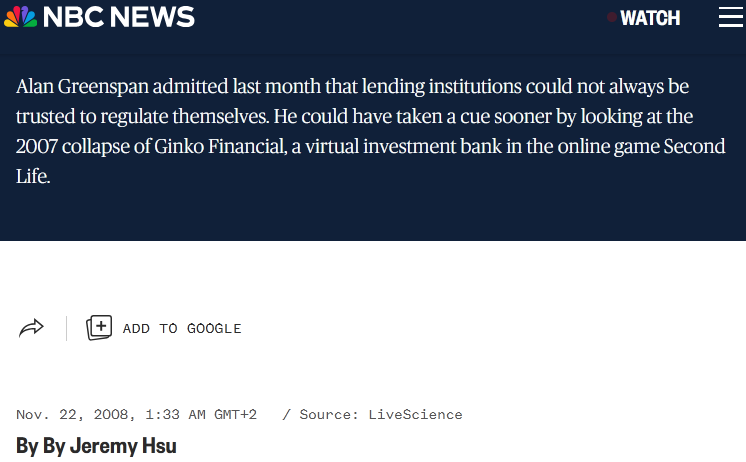
\includegraphics[width=3.125in,height=\textheight,keepaspectratio,alt={Post-mortem article from CBC detailing the 2007 crash of the virtual life economy caused by a virtual bank called Ginko Financial. Regulations outlawing virtual banks and allowing only real life banks to operate subsequently followed the event.}]{images/paste-3.png}\\
  \autocite{hsuSecondLifeBank2008}\strut \\
  At the end a food for thought ending. ``These are examples of whether
  to disregard human dignity and the rights they demand simply because
  their values and sense of being are commodified in a data stream. Some
  people might not take these seriously however this is worth thinking
  about the sentimental data forms people have that may not be this
  Second Life game.''\\
\end{itemize}

\subsection{Node 1.2: The Social Complacency of Multiplayer Games
Virtual
Evil}\label{node-1.2-the-social-complacency-of-multiplayer-games-virtual-evil}

\begin{itemize}
\item
  \textbf{Provocative Hook}: How do video game UIs turn ordinary gamers
  into cold, button-pushing virtual war criminals?
\item
  \textbf{Core IE Motivated Argument}: In MMOGs and strategy games
  (\emph{Defcon}, \emph{EVE Online}), games reward mechanical efficiency
  (points, numbers going up) while stripping away semantic feedback
  which
  \autocite{sicartHowLearnedLove2008a,sicartBanalitySimulatedEvil2009a}
  refers to as the ``banality of simulated evil''. Rule engines abstract
  human suffering into UI metrics, players become unthinking bureaucrats
  of virtual destruction \autocite{sicartBanalitySimulatedEvil2009a}.
  While not leading to overt evil in the Infosphere as defined by
  Floridi \autocite{himmaHandbookInformationComputer2008}, this suggests
  players are rewarded for lack of deep reflection, background static of
  moral numbness. This culture becomes reinforced through online
  multiplayer play, beyond similar single player games.
\item
  \textbf{Multi-Media Cue}:

  \begin{itemize}
  \tightlist
  \item
    Audio-visual node playing \emph{Defcon}'s nuclear strikes
    (minimalist radar + muffled crying audio) alongside real player
    voice-chats cheering for maximum kill counts
    \autocite{sicartHowLearnedLove2008a}.
  \end{itemize}
\end{itemize}

\section{Sub-Topic 2: Does Violence in MMOGs Impact Real Life?
(\textasciitilde300
Words)}\label{sub-topic-2-does-violence-in-mmogs-impact-real-life-300-words}

\subsection{Node 2.1: Does Violence in MMOGs Impact Real Life?
Considerations Over Varying Scopes (\textasciitilde300
Words)}\label{node-2.1-does-violence-in-mmogs-impact-real-life-considerations-over-varying-scopes-300-words}

\begin{itemize}
\item
  \textbf{Provocative Hook}: Crime rates drop as game sales rise---so
  why are we still obsessed with virtual slaughter?
\item
  The ``contamination thesis'' asserts game violence leaks into
  real-world aggression \autocite{goergerValueViolenceEthics2017a}.
  However, macro-data disproves the ``contamination thesis'' (games do
  not turn players into real-world mass shooters)
  \autocite{goergerValueViolenceEthics2017a,schulzkeDefendingMoralityViolent2010a}.
  However, macro-crime analysis miss cultural context
  \hyperref[node-2.3-satire-tragedy-vs.-atrocity-porn-the-endorsement-view]{Node
  2.3: Satire, Tragedy vs.~Atrocity Porn (The Endorsement View)}, and
  more microscopic lenses where changes can be induced or correlated
  with certain individuals. Schulzke and Ostritsch argue games operate
  inside a ``magic circle'' where virtual actions lack victims
  \autocite{ostritschAmoralistChallengeGaming2017a,schulzkeDefendingMoralityViolent2010a}.
  The moral question then shifts to whether a game \emph{glorifies}
  depravity or \emph{forces critical reflection}
  \autocite{goergerValueViolenceEthics2017a,sicartBanalitySimulatedEvil2009a}.
  Violent games contain nuanced, non-uniform nature. Further they do not
  automatically force so much as reveal the nuanced, non-uniform tastes
  of \emph{their player}; how they handle learning from the moral
  experiences presented in the game, and comment introspectively upon
  their own nature relative to the game.

  \begin{itemize}
  \tightlist
  \item
    Link to
    \hyperref[node-1.2-the-social-complacency-of-multiplayer-games-virtual-evil]{Node
    1.2: The Social Complacency of Multiplayer Games Virtual Evil}: Some
    players might display boredom in terms of ethical engagement and
    engage with the game for other reasons they do not introspect upon.
  \end{itemize}
\item
  \textbf{Multi-Media Cue}: Interactive slider charting video game sales
  against youth violent crime rates over 30 years (showing inverse
  correlation)\autocite{schulzkeDefendingMoralityViolent2010a}.

  \begin{itemize}
  \item
    Simple interaction idea is to hide each year of the graph either
    with the slider or by clicking the chart to reveal more years.
    Everytime they increase the slider or click to reveal, they see the
    amount of crime for that year.
  \item
    Before they click, they are asked to guess whether they think it
    will decrease or increase for the next year.
  \item
    They are then told they can research more if their guess was wrong
    and they want to learn why, with a link to where the chart is from.
  \end{itemize}
\end{itemize}

\subsection{Node 2.2: Games as Virtue
Scaffolding}\label{node-2.2-games-as-virtue-scaffolding}

\begin{itemize}
\item
  \textbf{Provocative Hook}: Can playing a violent game make you a
  \emph{more} virtuous person
  \autocite{schulzkeDefendingMoralityViolent2010a}?
\item
  \textbf{Core Argument \& Theoretical Connection}: Wonderly uses Humean
  sentimentalism to argue ultra-violent gaming erodes empathy
  \autocite{wonderlyHumeanApproachAssessing2008a} Rebutting this,
  Schulzke demonstrates via Kant that virtual attacks carry no intent to
  harm real people \autocite{schulzkeDefendingMoralityViolent2010a}, and
  via Aristotle that choice-engine games (\emph{Fallout 3}, \emph{The
  Last of Us}) serve as moral simulators to practice virtuous
  decision-making
  \autocite{goergerValueViolenceEthics2017a,schulzkeDefendingMoralityViolent2010a}
\item
  \textbf{Multi-Media Cue}: Decision-tree node showing the moral
  dilemmas from \emph{Fallout 3} OR \emph{The Witcher Series}, showing
  how moral engines scaffold ethical reflection.
\end{itemize}

\subsection{Node 2.3: Satire, Tragedy vs.~Atrocity Porn (The Endorsement
View)}\label{node-2.3-satire-tragedy-vs.-atrocity-porn-the-endorsement-view}

\begin{itemize}
\item
  \textbf{Provocative Hook}: Why is torturing in \emph{GTA V}
  satirically defensible, but playing \emph{KZ Manager} morally
  abhorrent \autocite{ostritschAmoralistChallengeGaming2017a}?
\item
  \textbf{Core Argument \& Theoretical Connection}: Goerger and
  Ostritsch argue that graphic nature alone does not dictate morality;
  context and value integration do
  \autocite{goergerValueViolenceEthics2017a,ostritschAmoralistChallengeGaming2017a}.
  Under Ostritsch's \emph{Endorsement View}, representing evil
  (\emph{GTA V}) is not immoral if framed satirically, as moral tragedy
  (\emph{The Last of Us}, \emph{The Witcher 3}), whereas endorsing an
  abhorrent worldview (\emph{KZ Manager}, \emph{Hatred, RapeLay})
  violates moral obligations
  \autocite{ostritschAmoralistChallengeGaming2017a}.
\item
  \textbf{Multi-Media Cue}:

  \begin{itemize}
  \item
    PANE 1 - Poll and discussion: \textbf{{[}30-Second Timer{]}}
    \emph{``In 1989, a text-and-graphic game} \textbf{KZ Manager}
    \emph{was secretly distributed on Commodore 64 floppy disks across
    Europe. Players managed resources, bought gas and optimized the
    efficiency of a Nazi concentration camp. It was notoriously banned.
    Do you agree with the ban.''}

    \begin{itemize}
    \item
      Information Ethical Idea board: Some games show ethical
      degradation itself as part of the educational game experience.
      This requires tact from authors to avoid encouraging harm
      endorsement over real groups, retraumatizing them, or without
      asking affected specifically targeted groups how they would like
      to be portrayed if high impersonations of them are used.

      \begin{itemize}
      \tightlist
      \item
        Do you think this contrasts acceptable games that endorse
        non-specific harms on non-specific groups? Would a game like GTA
        be more socially acceptable due to this, are there specific
        violations within the game.
      \end{itemize}
    \end{itemize}
  \item
    PANE 2 - Discussion \emph{then} poll:

    \begin{itemize}
    \item
      Why do we freely play historical war games where we slaughter
      ancient Romans, Spartans, or 18th-century soldiers, but recoil at
      games depicting recent genocides or the Holocaust? How much
      \emph{time} or \emph{generational distance} must pass before real
      human trauma becomes ``acceptable'' material for a game engine?
      Does this require being sensitive to human collective trauma much
      like temperature?
    \item
      Reveal a game: \emph{RapeLay. The banned, originally on Amazon's
      website, was a 2006 Japanese adult PC game required players to
      stalk and simulate the rape of a mother and her two daughters,
      earning points for acts of sexual violence, including tailing
      victims on commuter trains and forcing them to have abortions.}

      \begin{itemize}
      \item
        Are some harms eternal thematic human experiences. No amount of
        time will alter acceptance of concepts that are not historical
        and exist always as harms. Without arguing about the law, of
        ``should'' the game be banned, we argue about the information
        ethical nature.
      \item
        Is it a reflection of ethical decay or depravity if a gamer
        ignores the person hood of the people and healthier ways of
        consuming their experiences in data-ified form.
      \end{itemize}
    \end{itemize}
  \item
    PANE 3: Closing Discussion:

    \begin{itemize}
    \item
      Do you align with \textbf{Ostritsch's Endorsement View} (that
      endorsing real-world evil through game mechanics is an actual
      moral failure, not just a virtual one)?
    \item
      Or do you align with \textbf{Schulzke's Kantian/First Amendment
      defense} (that as long as no real living person is harmed in the
      ``magic circle,'' censorship over an individual's historical or
      present day harm endorsements is a greater moral danger than
      repulsive pixel art).
    \end{itemize}
  \end{itemize}
\end{itemize}

\section{References}\label{references}

\printbibliography[heading=none]





\end{document}
